% Exercise ID: MAT_P4FUNCOE_4FIN_GRA_002
% Exercise ID: MAT_P4FUNCOE_4FIN_GRA_002
% Module: MÓDULO P4 - Funções | Concept: Função Inversa | Type: Determinação Gráfica
% Difficulty: 2/5 (Fácil) | Type: desenvolvimento
% Points: 10 | Time: 10 min
% Tags: inversa, grafico, simetria, funcao_quadratica
% Author: Professor | Date: 2025-11-18
% Status: active
% Description: Dado o gráfico de ramos de funções, desenhar o gráfico da inversa

\exercicio
Na figura está representado o gráfico de uma função $h$ definida em $]-\infty, 0]$. Represente, no referencial dado, o gráfico da função inversa $h^{-1}$.

\begin{figure}[ht]
\centering
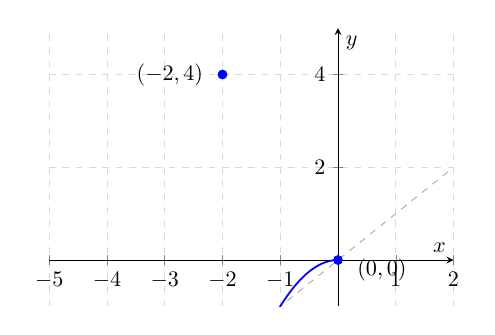
\begin{tikzpicture}[scale=0.8]
    \begin{axis}[
        axis lines = middle,
        xlabel = $x$,
        ylabel = $y$,
        xmin = -5, xmax = 2,
        ymin = -1, ymax = 5,
        grid = major,
        grid style = {dashed, gray!30},
        width = 8cm,
        height = 6cm,
    ]
    \addplot[domain=-5:5, dashed, gray!70, thin] {x};
    
    \addplot[domain=-4:0, samples=100, thick, blue] {-x^2};
    \addplot[mark=*, mark size=2pt, blue] coordinates {(0,0)};
    \addplot[mark=*, mark size=2pt, blue] coordinates {(-2,4)};
    \node[anchor=east] at (axis cs:-2.2,4) {$(-2,4)$};
    \node[anchor=north west] at (axis cs:0.2,0.2) {$(0,0)$};
    \end{axis}
\end{tikzpicture}
\end{figure}

\bigskip

\exercicio
Na figura está representado o gráfico de uma função $k$ definida em $[1, 5]$. Represente, no referencial dado, o gráfico da função inversa $k^{-1}$.

\begin{figure}[H]
\centering
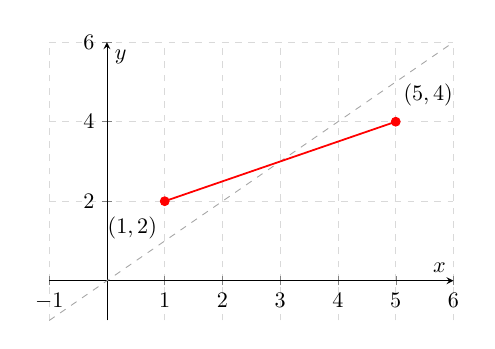
\begin{tikzpicture}[scale=0.8]
    \begin{axis}[
        axis lines = middle,
        xlabel = $x$,
        ylabel = $y$,
        xmin = -1, xmax = 6,
        ymin = -1, ymax = 6,
        grid = major,
        grid style = {dashed, gray!30},
        width = 8cm,
        height = 6cm,
    ]
    \addplot[domain=-1:6, dashed, gray!70, thin] {x};
    
    \addplot[domain=1:5, thick, red] {0.5*x+1.5};
    \addplot[mark=*, mark size=2pt, red] coordinates {(1,2)};
    \addplot[mark=*, mark size=2pt, red] coordinates {(5,4)};
    \node[anchor=south west] at (axis cs:5,4.2) {$(5,4)$};
    \node[anchor=north east] at (axis cs:1,1.8) {$(1,2)$};
    \end{axis}
\end{tikzpicture}
\end{figure}
\vspace{3cm}
}